% intro et déroulement du cours

\begin{frame}{Contenu du cours}
\begin{columns}
\begin{column}{0.6\textwidth}
\begin{itemize}
\item Modèles utilisés pour la synthèse d'images
\begin{itemize}
\item Synthèse d'images temps réel : le modèle d'OpenGL
\item Quelques idées sur la synthèse d'images hors ligne
\end{itemize}
\item Programmation OpenGL
\item Focus sur les shaders
\item Unity3D
\item Les graphes de scène
\item OpenSceneGraph
\end{itemize}
\end{column}
\begin{column}{0.39\textwidth}
\begin{center}
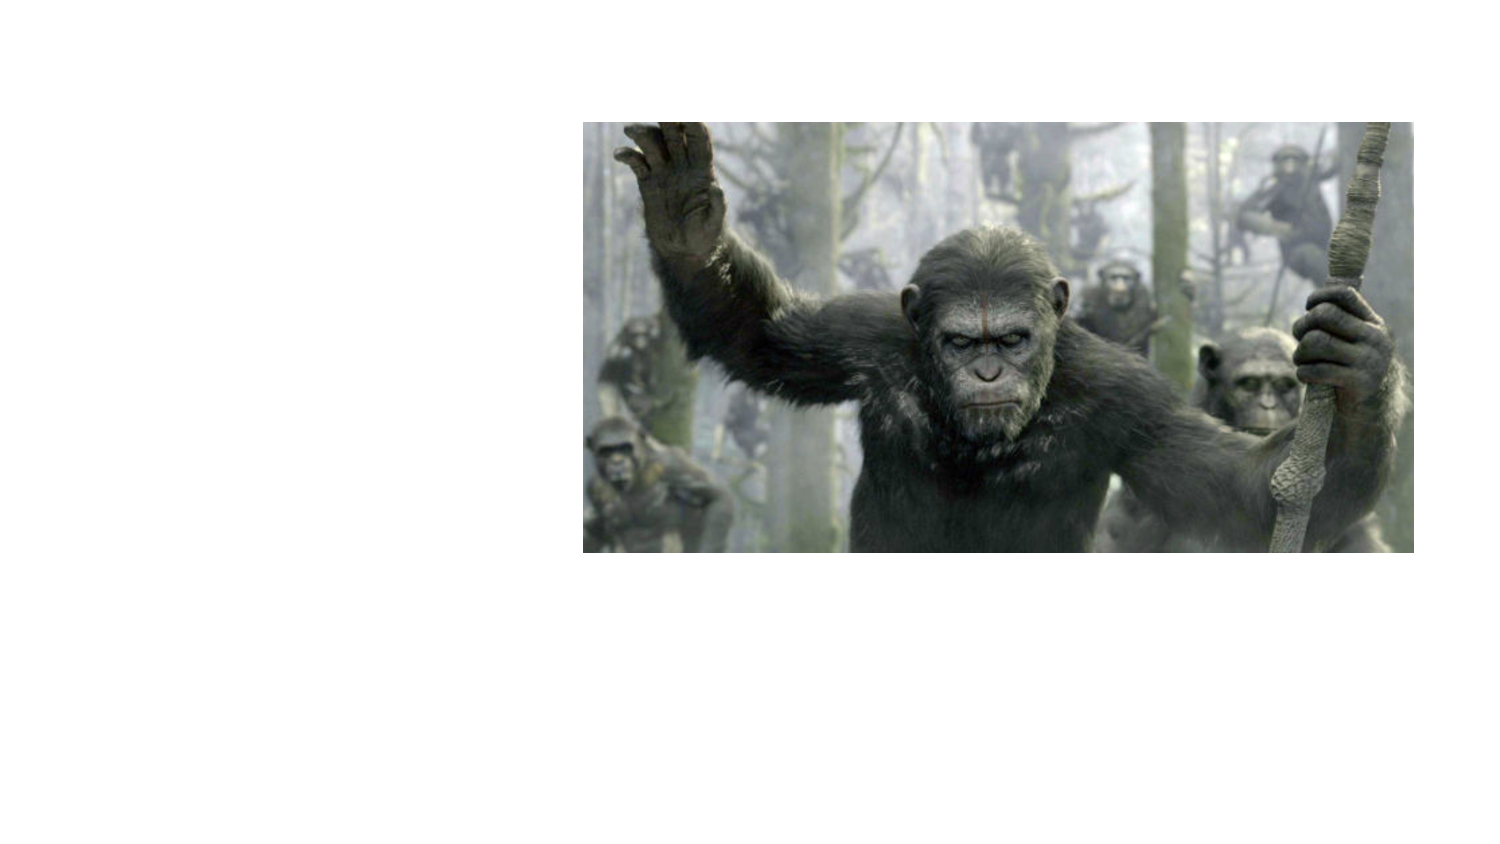
\includegraphics[width=\textwidth]{figs/apes.pdf}
\end{center}
\end{column}
\end{columns}
\end{frame}

\begin{frame}{Introduction}
\begin{center}
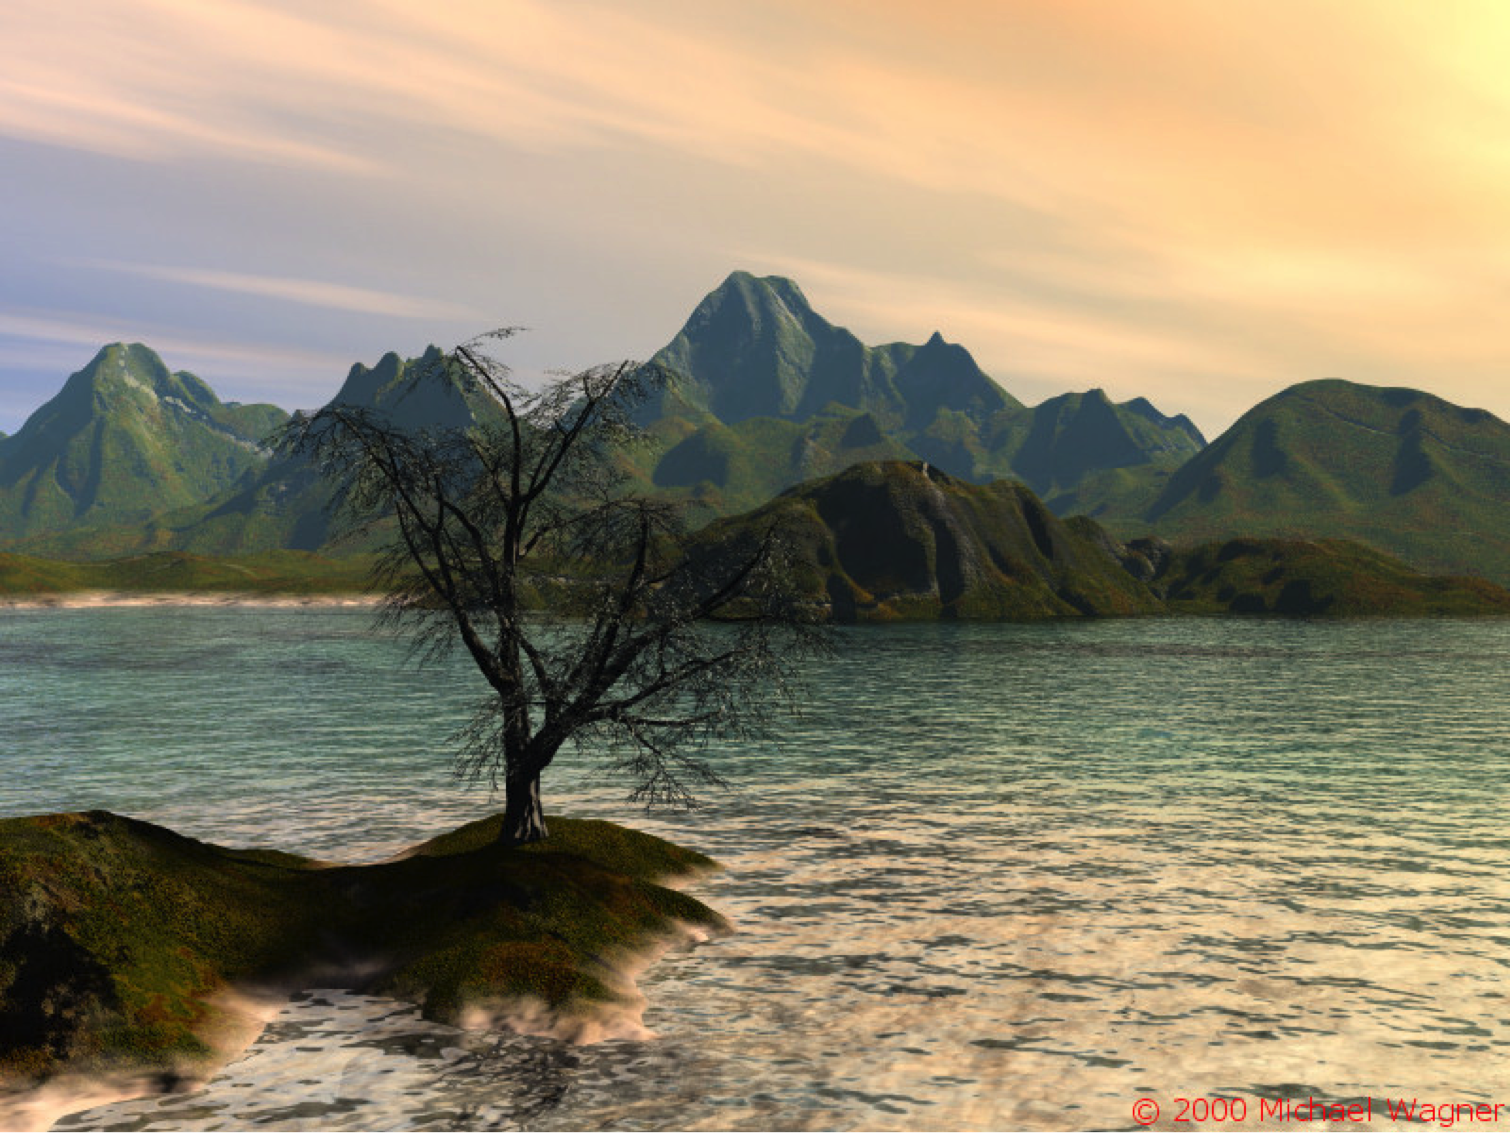
\includegraphics[height=\textheight]{figs/wagner00.png}
\emph{Dawn of the Planet of the Apes, 2014}
\end{center}
\end{frame}

\subsection{Petite histoire de la synthèse d'images}

\begin{frame}{Images de synthèse et cinéma (1/2)}
\begin{itemize}
\item 1976 : première apparition \textit{Future World}
\item 1982 : pendant tout le film \textit{Tron}
\item 1984 : se veut réaliste \textit{Last Star Fighter}
\item 1988 : premier Oscar \textit{Tin Toy}
\item 1989 : avec des êtres vivants \textit{Abyss}
\end{itemize}
\begin{center}
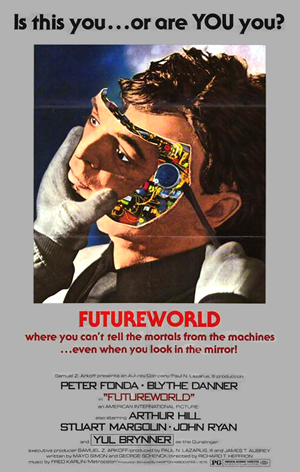
\includegraphics[height=0.28\textheight]{figs/Futureworld.jpg}
\hspace{0.1cm}
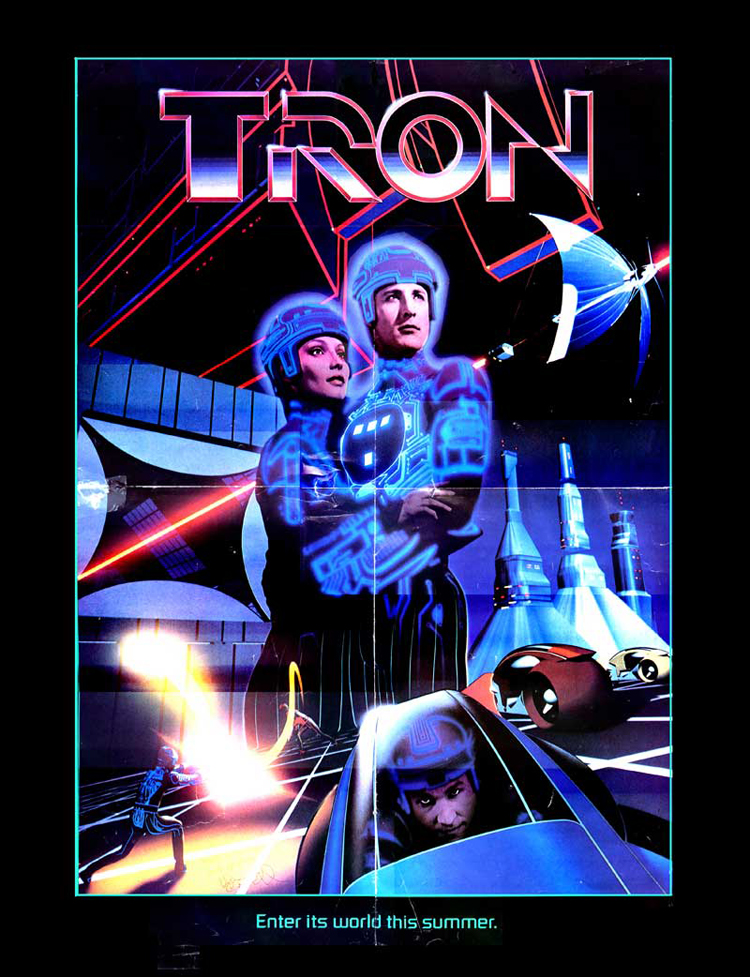
\includegraphics[height=0.28\textheight]{figs/Tron1982.jpg}
\hspace{0.1cm}
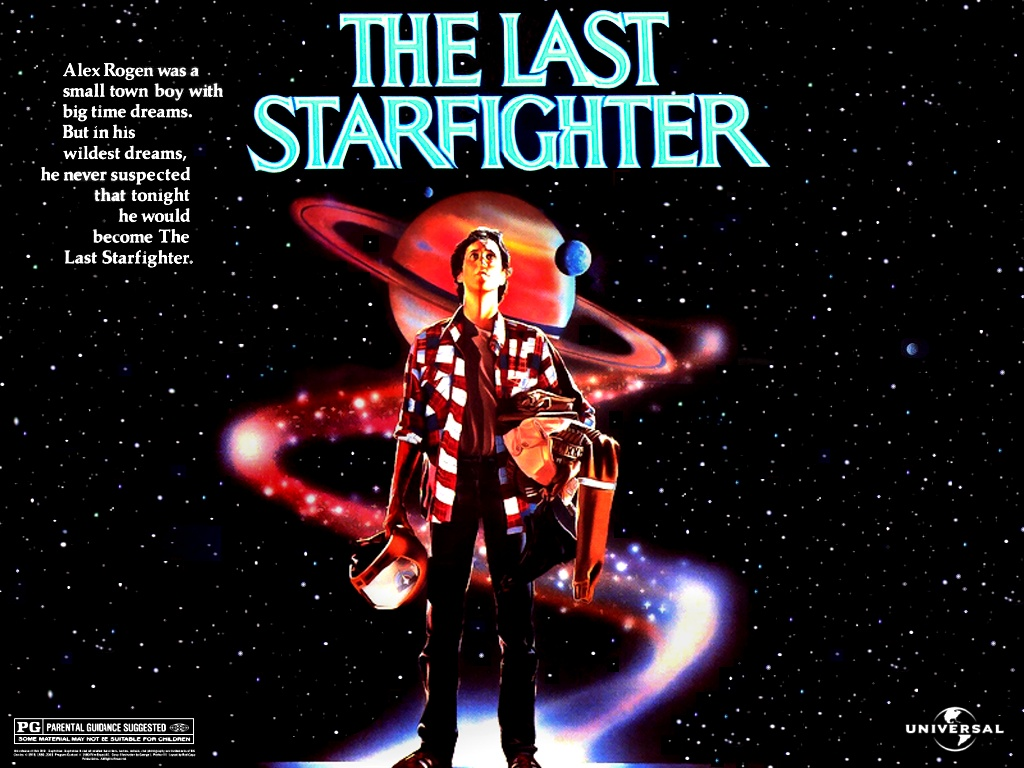
\includegraphics[height=0.28\textheight]{figs/thelaststarfighter.jpg}
\hspace{0.1cm}
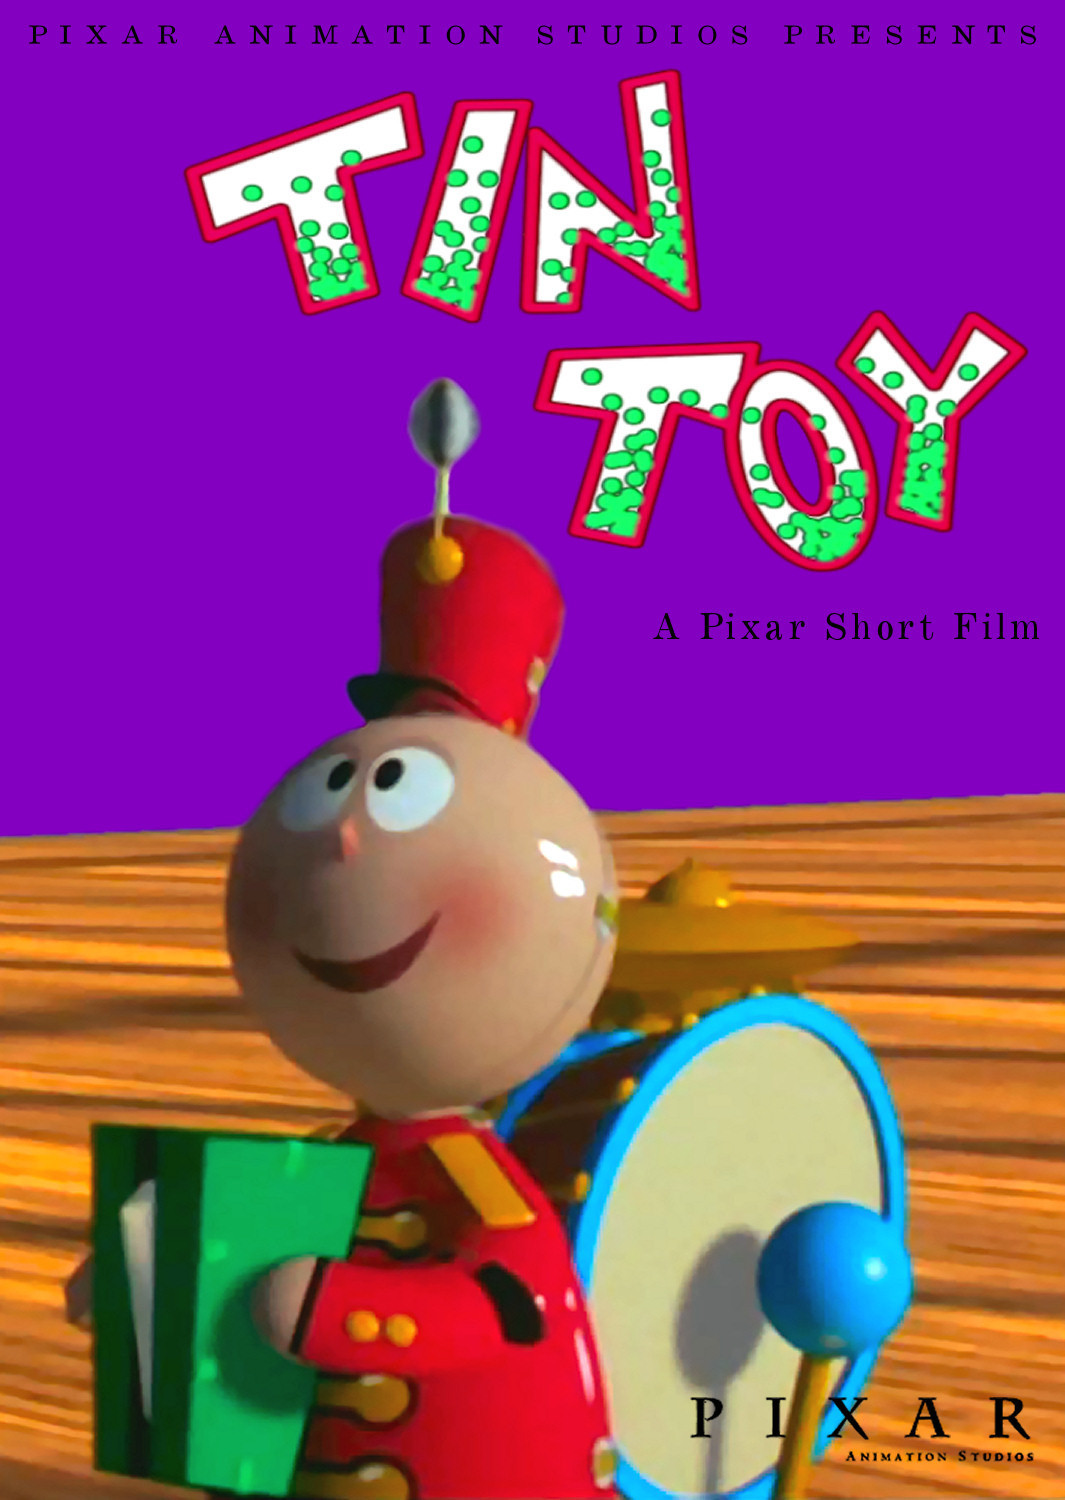
\includegraphics[height=0.28\textheight]{figs/tintoy.jpg}
\hspace{0.1cm}
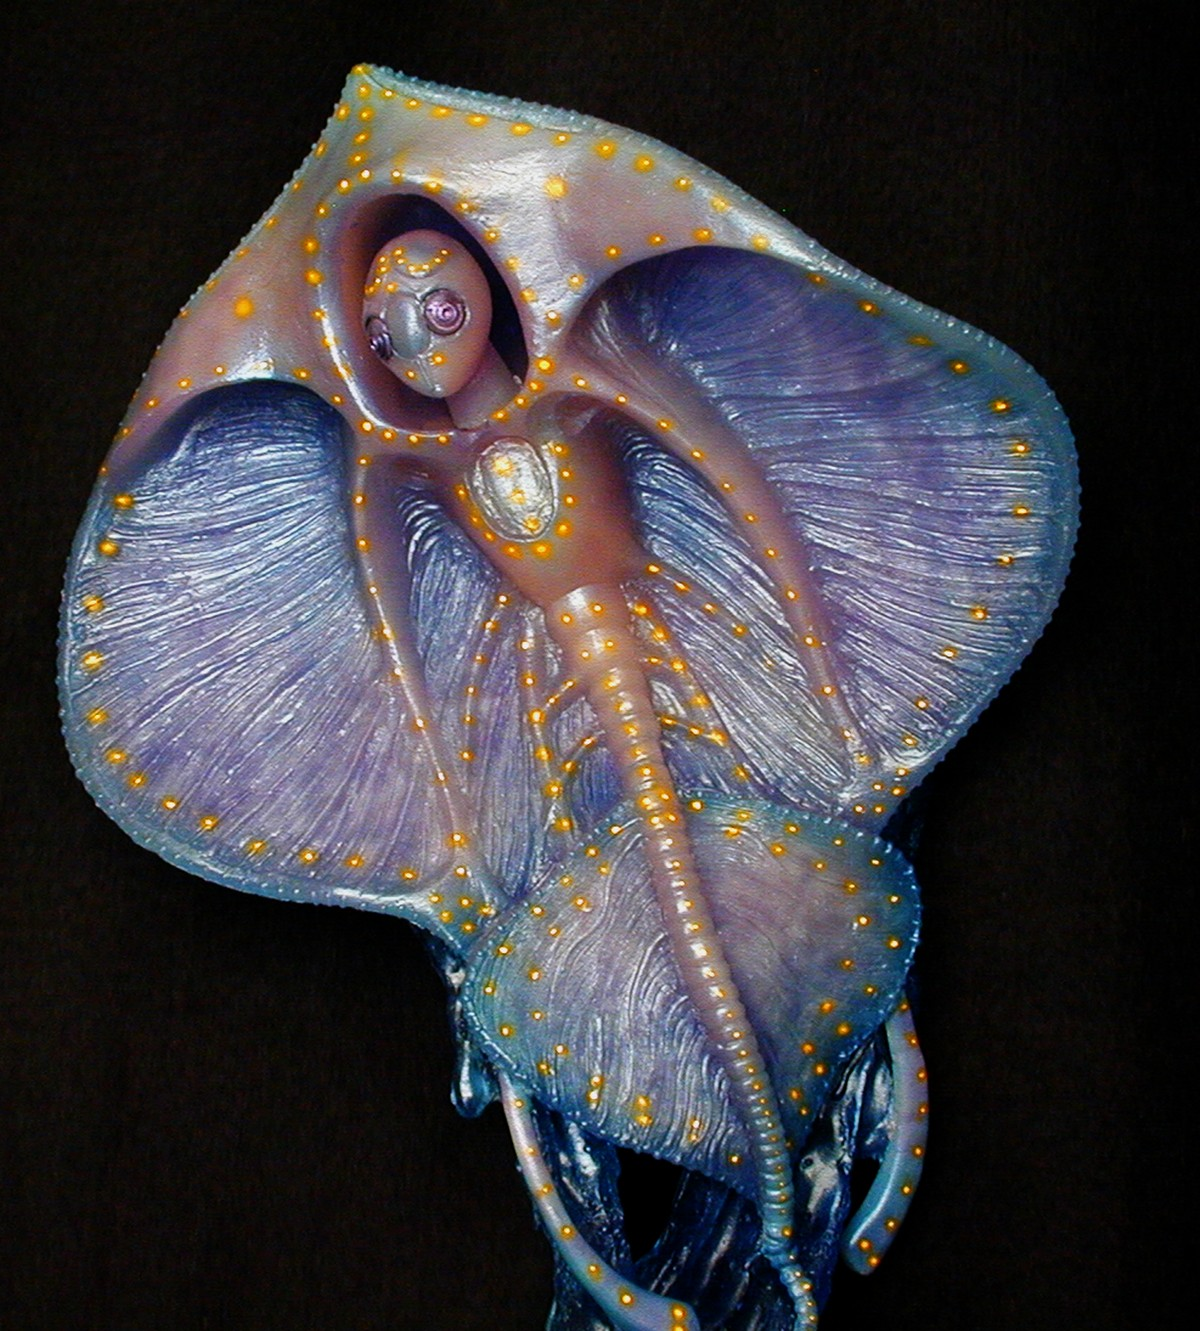
\includegraphics[height=0.28\textheight]{figs/abyss.jpg}
\end{center}
\end{frame}

\begin{frame}{Images de synthèse et cinéma (2/2)}
\begin{itemize}
\item 1993 : premières créatures connues \textit{Jurassic Park}
\item 1982 : doublures d'acteurs \textit{Batman returns}
\item 1984 : 3D de synthèse intégrale \textit{Toy Story}
\item Et ça continue...
\end{itemize}
\begin{center}
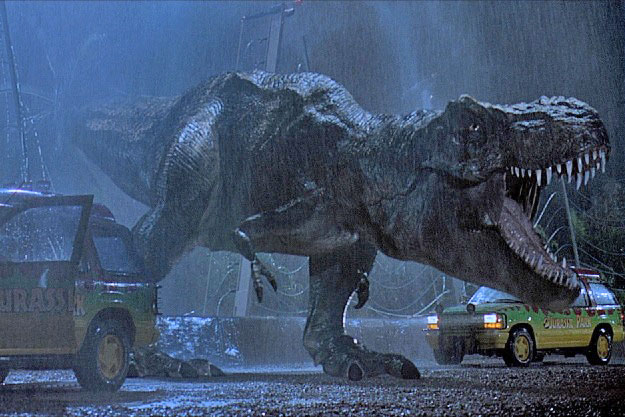
\includegraphics[height=0.28\textheight]{figs/Jurassic-Park.jpg}
\hspace{0.1cm}
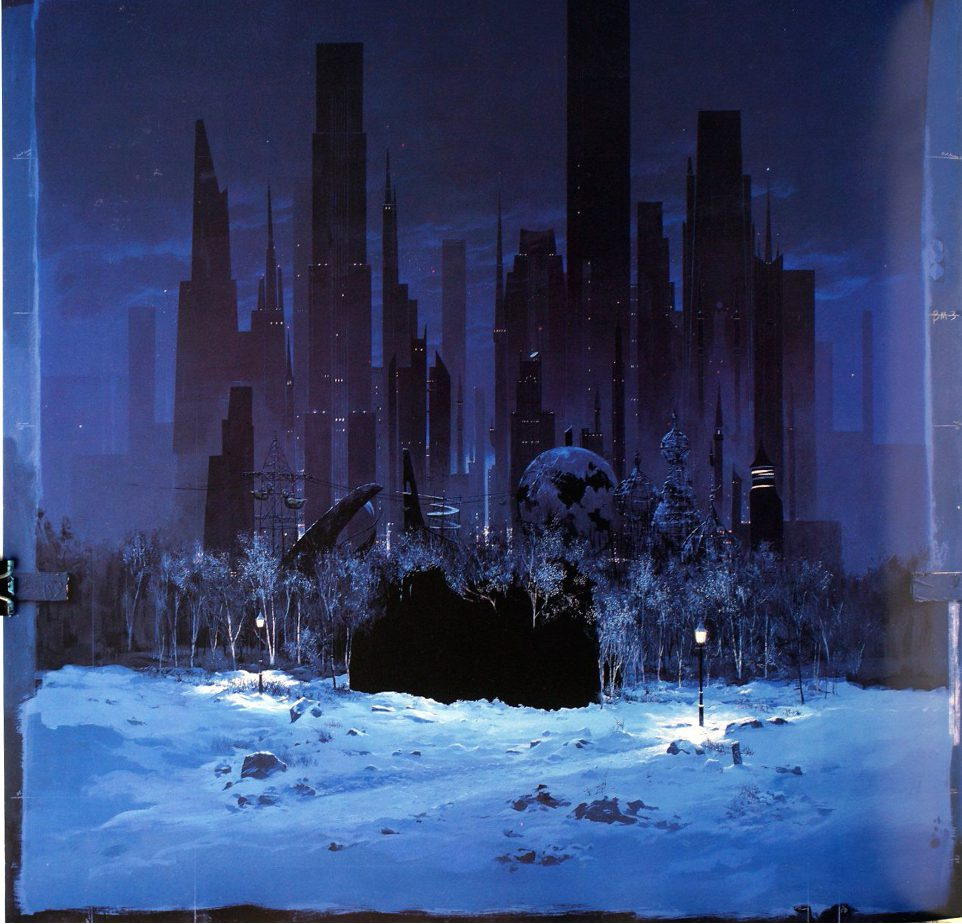
\includegraphics[height=0.28\textheight]{figs/BatmanReturns.jpg}
\hspace{0.1cm}
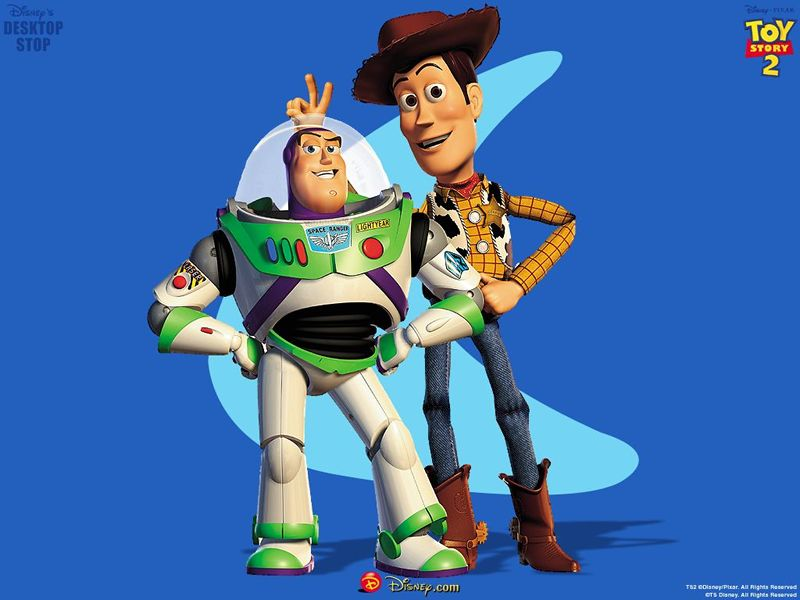
\includegraphics[height=0.28\textheight]{figs/ToyStory.jpg}
\end{center}
\end{frame}

\begin{frame}{Rappel}
\begin{itemize}
\item Dans ce cours, on s'intéresse la plupart du temps à la synthèse d'images en temps réel
\begin{center}
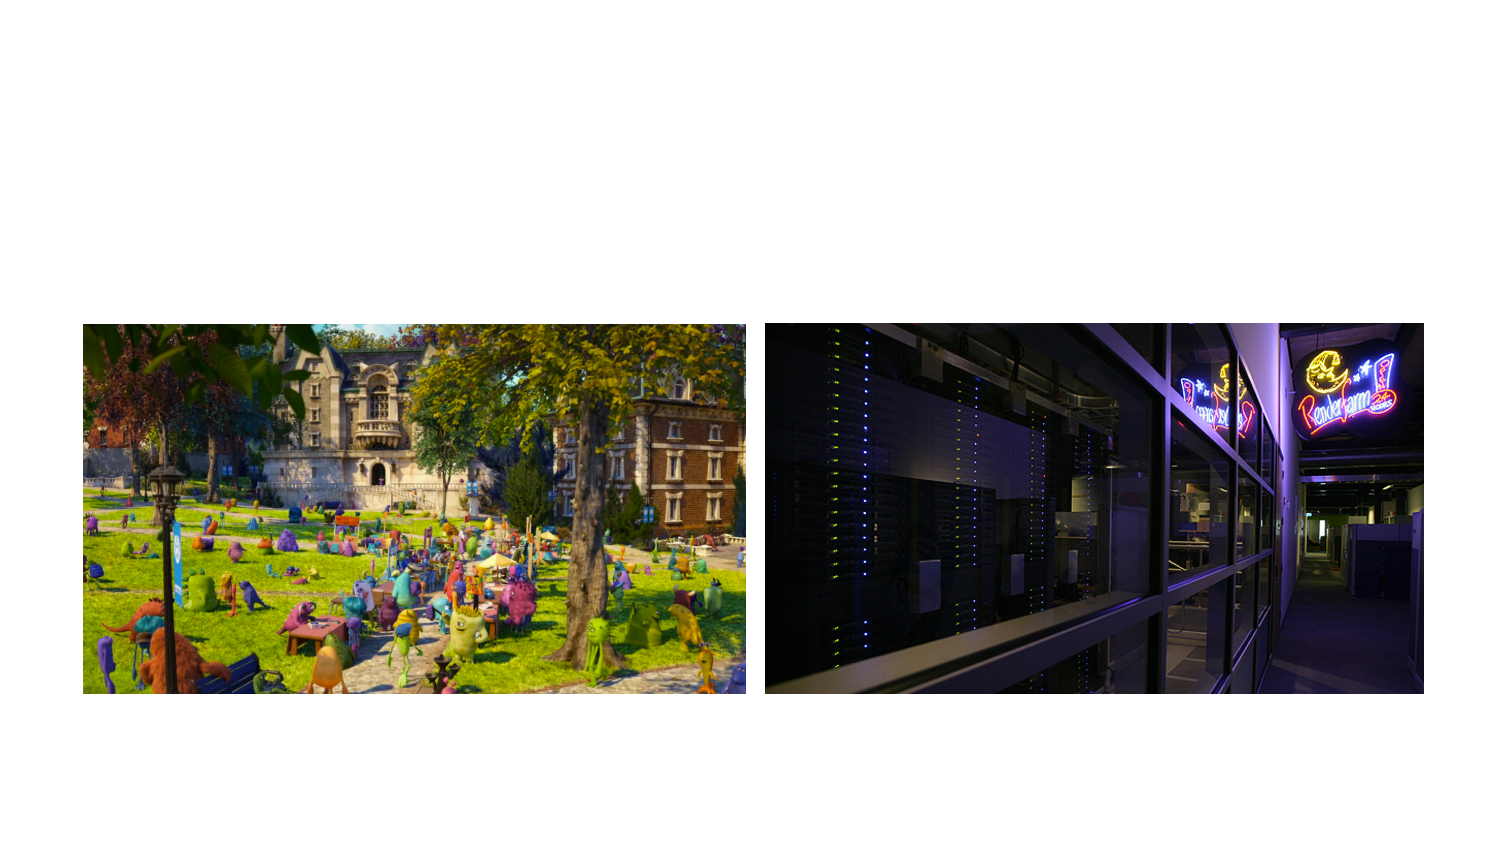
\includegraphics[width=.9\textwidth]{figs/monsters.pdf}
\end{center}
\item 1 image de \textit{Monstres Academy} : 29h de calcul sur une ferme de 24000 c\oe urs !
\end{itemize}
\end{frame}

\begin{frame}{Eléments de bibliographie}
\begin{itemize}
\item Livres
\begin{itemize}
\item Informatique graphique et rendu. B. Péroche, D. Bechmann (Eds). Hermès, 2007.
\item 3D Computer Graphics. A. Watt, Addison-Wesley, 1999. 642 pages !
\item Computer Graphics, Principles and Practice. J. Hughes, A. van Dam, M. McGuire, D. Sklar, J. Foley, S. Feiner, K. Akeley. Addison-Wesley, 2013. 1264 pages. La suite du \textit{Foley et van Dam}.
\end{itemize}
\item Revues scientifiques
\begin{itemize}
\item ACM SIGGRAPH : salon professionnel, conférence scientifique
\item ACM Transactions on Graphics
\end{itemize}
\item Cours en ligne
\begin{itemize}
\item Coursera : \url{https://www.coursera.org/course/interactivegraphics}
\item EdX : \url{https://www.edx.org/course/uc-berkeleyx/uc-berkeleyx-cs-184-1x-foundations-1003}
\item OpenCourseWare \url{http://ocw.mit.edu/courses/electrical-engineering-and-computer-science/6-837-computer-graphics-fall-2012/}
\end{itemize}
\end{itemize}
\end{frame}
